%   % !TEX root = ../../VIII,3_Rahmen-TeX_8-1.tex
%
%
%   Band VIII, 3 N.~??S01.03
%   Signatur/Tex-Datei: LH_35_09_23_004-005
%   RK-Nr. 41208 /3
%   \ref{dcc_02-2}
%   Überschrift: De corporum concursus scheda secundo-secunda
%   Modul: Mechanik / Stoß ()
%   Datierung: [Januar 1678]
%   WZ: LEd-WZ 803017 = RK-WZ 1264 (eins)
%   SZ: %\leibdashv %\leibvdash %\groesser %\kleiner (vier)
%   Bilddateien (PDF): LH_35_09_23_004-005_d1; LH_35_09_23_004-005_d2 (insgesamt: zwei)
%   Verzeichniseinträge: vollständig
%   \textls{} statt \textso{} (Ausnahme: Personenverzeichnis)
%
%
\selectlanguage{ngerman}%
\frenchspacing%
%
\begin{ledgroupsized}[r]{120mm}%
\footnotesize%
\pstart%
\noindent\textbf{Überlieferung:}%
\pend%
\end{ledgroupsized}%
\begin{ledgroupsized}[r]{114mm}%
\footnotesize%
\pstart%
\parindent -6mm
\makebox[6mm][l]{\textit{L}}%
Konzept: LH XXXV 9, 23 Bl.~4\textendash5.
Ein Bogen 2\textsuperscript{o},
im Textträger von N.~\ref{dcc_02-1} %??S01\textsubscript{2} 
umschlossen;
ein Wasserzeichen auf Bl.~4.
Vier Seiten;
Textfolge (nur zum Teil von Leibniz festgelegt): Bl.~4~r\textsuperscript{o}, 5~r\textsuperscript{o}, 4~v\textsuperscript{o}\! und 5~v\textsuperscript{o}; 
% und 4~r\textsuperscript{o};
ein Kustos am Ende von Bl.~4~v\textsuperscript{o} verweist auf den Anfang von Bl.~5~v\textsuperscript{o}.
Bl.~4~r\textsuperscript{o} ist um drei Viertel leer;
Bl.~5~r\textsuperscript{o} ganz gestrichen.
%Am Kopf von Bl.~4~r\textsuperscript{o} Satzfragment von Leibnizens Hand, offenbar mit dem Text auf Bl.~5~v\textsuperscript{o} zusammenhängend und folglich erst nach Abfassung von N.~\ref{dcc_08} %??S01\textsuperscript{10}
%hinzugefügt:
%\textit{$am^2$ aequ. $b^2.$}
%\lbrack/\rbrack\
%\textit{Si ponamus viam centri gravitatis\protect\index{Sachverzeichnis}{centrum gravitatis} manere eandem
%\sout{et vero constat esse}
%pariter ac distantiam}\lbrack,\rbrack\
%\textit{habebimus has duas aequationes
%\sout{quando}
%$a\epsilon^2 + by^2$ aequ. $ae^2$ et a} \lbrack\textit{bricht ab.}\rbrack\ 
N.~\ref{dcc_02-2} %??S01\textsubscript{3} 
knüpft inhaltlich an N.~\ref{dcc_02-1} %??S01\textsubscript{2} 
(S.~\pageref{LH_35_09_23_006r_MargDeIIoIIa}) an;
eine Randbemerkung weist dort auf den Zusammenhang mit N.~\ref{dcc_02-2} %??S01\textsubscript{3} 
hin.
Siehe zur Textgenese von N.~\ref{dcc_02-2} die editorische Vorbemerkung, S.~\refpassage{dcc_intro_II-II_gdr-1}{dcc_intro_II-II_gdr-2}.
\pend%
\end{ledgroupsized}%
%
\begin{ledgroupsized}[r]{114mm}%
\footnotesize%
\pstart%
\parindent -6mm%
\makebox[6mm][l]{\textit{E}}%
\textsc{Fichant},\cite{01056} 1994, S.~89\textendash92 (mit kommentierter französischer Übersetzung, S. 208\textendash212).
\pend%
\end{ledgroupsized}%
%
\selectlanguage{latin}%
\frenchspacing%
\count\Bfootins=1100%
\count\Afootins=1200%
\count\Cfootins=1100%
%
\vspace{8mm}
\pstart%
\normalsize%
\noindent%
%
\lbrack4~r\textsuperscript{o}\rbrack% % % %  Blatt 4r
%
\hspace{41mm}%
Scheda secundo-secunda%
\protect\index{Sachverzeichnis}{scheda}
\pend%
\vspace{0.5em}%
%
\pstart%
\noindent%
Nota\lbrack:\rbrack\
%
\edlabel{LH_35_09_23_004-005_Blatt4r-1}%
% \edlabel{LH_35_09_23_004-00_concursu12}%
\edtext{haec scheda%
\protect\index{Sachverzeichnis}{scheda}}{%
\lemma{haec scheda}\Cfootnote{%
Damit könnte auch die \textit{Scheda II} (N.~\ref{dcc_02-1}%??S01\textsubscript{2}
) gemeint sein, mit der N.~\ref{dcc_02-2} %??S01\textsubscript{3}
sowohl der Überlieferung nach wie auch inhaltlich zusammenhängt.% (siehe oben, die \textit{Überlieferung}).
}}
%
recte concludit non posse
%
\edtext{servari centri gravitatis viam%
\protect\index{Sachverzeichnis}{via centri gravitatis}%
}{%
\lemma{servari}\Bfootnote{%
\textit{(1)}~centrum gravitatis et
\textit{(2)}~centri gravitatis viam%
~\textit{L}}}
%
eandem,
aut eandem distantiam,%
\protect\index{Sachverzeichnis}{distantia corporum}
posita eadem semper quantitate motus.%
\protect\index{Sachverzeichnis}{quantitas motus}
Verum absolute male concludit
quod distantia et via centri non serventur,
falsa est enim
\edtext{hypothesis Cartesiana%
\protect\index{Namensregister}{\textso{Descartes} (Cartesius, des Cartes), René 1596\textendash1650}%
\protect\index{Sachverzeichnis}{hypothesis Cartesiana}
de servanda motus quantitate.%
\protect\index{Sachverzeichnis}{quantitas motus servanda}%
}{%
\lemma{hypothesis \lbrack...\rbrack\ quantitate}\Cfootnote{%
Vgl. R.~\textsc{Descartes}, \cite{00035}\textit{Principia philosophiae}, pars~II, % §~36 (Amsterdam 1644, S.~53\,f.; \cite{00120}\textit{DO} VIII,~1, S.~61\,f.).
§§~40\textendash43 (Amsterdam 1644, S.~57\textendash59; \cite{00120}\textit{DO} VIII.1, S.~65\textendash67).}}%
\edlabel{LH_35_09_23_004-005_Blatt4r-2}
\pend%
\vspace{1.0em}%
%
\pstart%
\noindent%
\lbrack\textit{Textfragment am Rand von Bl.~4~r\textsuperscript{o}, mit dem Text auf Bl.~5~v\textsuperscript{o} zusammenhängend:}\rbrack\
\pend%
\vspace{0.5em}%
%
\pstart%
\noindent%
$am^2$ aequ. $b^2.$
% \lbrack/\rbrack\
Si ponamus viam centri gravitatis%
\protect\index{Sachverzeichnis}{centrum gravitatis}
manere
%
\edtext{eandem pariter ac distantiam}{%
\lemma{eandem}\Bfootnote{%
\textit{(1)}~et vero constat esse
\textit{(2)}~pariter ac distantiam%
~\textit{L}}}%
%
\lbrack,\rbrack\
habebimus has duas
%
\edtext{aequationes%
\protect\index{Sachverzeichnis}{aequatio}
$a\epsilon^2 + by^2$ aequ. $ae^2$ et \textit{a}%
}{%
\lemma{aequationes}\Bfootnote{%
\textit{(1)}~quando
\textit{(2)}~$a\epsilon^2 + by^2$ aequ. $ae^2$ et \textit{a}%
~\textit{L}}}
\lbrack\textit{bricht ab.}\rbrack\ 
%
\lbrack5~r\textsuperscript{o}\rbrack% % % %  Blatt 5r
%
\pend%
%\vspace{2.5em}%
%
%
%  \newpage% 
  \vspace{1.5em}%	% Diagramm Fig.~1
  \centerline{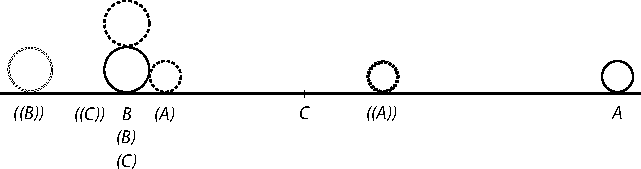
\includegraphics[width=0.76\textwidth]{gesamttex/edit_VIII,3/images/LH_35_09_23_004-005_d1.pdf}}%
  \vspace{0.5em}
  \centerline{\lbrack\textit{Fig.~1, gestr.}\rbrack}%
%  \label{LH_35_09_23_005r_Fig.1}%
%  \vspace{1.5em}%
  \newpage%
%
%
\pstart%
\noindent%
\lbrack\textit{Nachfolgend kleingedruckter Text in L gestrichen:}\rbrack%
\pend%
\vspace{0.5em}%
%
%
\footnotesize%
\pstart%
\noindent%
\edtext{%
Cum%
\edlabel{LH_35_09_23_004-005_Blatt5r-1}
corpus minus%
\protect\index{Sachverzeichnis}{corpus minus in majus}
%
\edtext{\textit{A}}{%
\lemma{\textit{A}}\Bfootnote{\textit{erg.~L}}}
%
incurrit in majus\protect\index{Sachverzeichnis}{corpus incurrens}
%
\edtext{\textit{B}}{%
\lemma{\textit{B}}\Bfootnote{%
\textit{erg.~L}}}
%
certum est minus repelli,%
\protect\index{Sachverzeichnis}{corpus repulsum}
videamus saltem an hoc conciliari possit
cum via centri gravitatis eadem manente.%
\protect\index{Sachverzeichnis}{via centri gravitatis}}{%
\lemma{Cum \lbrack...\rbrack\ manente}\Cfootnote{%
Siehe N.~\ref{dcc_02-1}, %??S01\textsubscript{2}, 
S.~\refpassage{LH_35_09_23_006r_viacentrigrav_vlai-1}{LH_35_09_23_006r_viacentrigrav_vlai-2}; \refpassage{LH_35_09_23_006r_viacentrigrav_mesj-1}{LH_35_09_23_006r_viacentrigrav_mesj-2}.}}
%
Nam quando corpus majus incurrit in minus%
\protect\index{Sachverzeichnis}{corpus majus in minus}
eadem manet via centri%
\protect\index{Sachverzeichnis}{centrum gravitatis}
%
\edtext{gravitatis.%
\protect\rule[-3mm]{0pt}{6mm}
\newline%
\indent%
\textit{A(A)} aequ. \textit{AB} aequ. \textit{A(B)} aequ. \textit{A(C)} aequ. \textit{e}.}{%
\lemma{gravitatis.}\Bfootnote{%
\textit{(1)}~\textit{A(A)} via celeritas incursus vocetur \textit{e}. aequal. \textit{A}
\textit{(2)}~\textit{A(A)} aequ. % \textit{AB} aequ. \textit{A(B)} aequ. \textit{A(C)} 
\lbrack...\rbrack\ aequ. \textit{e}.%
~\textit{L}}}%
\rule[-3mm]{0pt}{6mm}
%
% \pend%
%
% \pstart%
% \rule[-3mm]{0pt}{6mm}%
%
\quad
$\displaystyle\frac{AC}{BC}$ aequ. $\displaystyle\frac{b}{a}$ et $AC+BC\, \sqcap\, e.$
%
Ergo $AC\, \sqcap\, e-BC$
et rursus \textit{AC} aequ.
\rule[-2mm]{0pt}{5mm}%
$\displaystyle\frac{b}{a}BC,$
ergo $e-BC\, \sqcap\, \displaystyle\frac{b}{a}BC$
seu \textit{BC} aequ.
$\displaystyle\frac{e}{1+\displaystyle\frac{b}{a}}$ aequ.
\rule[-2mm]{0pt}{5mm}%
$\displaystyle\frac{a}{a+b}e,$
et \textit{AC} aequ.
$\displaystyle\frac{b}{a+b}e,$
ergo et \textit{C(C)} aequ.
\rule[-2mm]{0pt}{5mm}%
$\displaystyle\frac{a}{a+b}e,$
%
est enim \textit{BC} aequ. \textit{C(C)}.
% \pend%
% %
% \pstart%
\quad
Ponamus jam et \textit{(C)((C))}
\rule[-2mm]{0pt}{5mm}%
%
\edtext{aequ. $\kappa,$
et corporum distantia%
\protect\index{Sachverzeichnis}{distantia corporum}
secunda \textit{((A))((B))} sit $\delta,$
patet}{%
\lemma{aequ. $\kappa,$}\Bfootnote{%
\textit{(1)}~patet esse
\textit{(2)}~et corporum distantia secunda \textit{((A))((B))} \textbar\ distantia \textit{gestr.} \textbar\ sit $\delta,$ patet%
~\textit{L}}}
%
fore \textit{((B))((C))} aequ.
\rule[-3mm]{0pt}{5mm}%
$\displaystyle\frac{a}{a+b}\delta$
et \textit{((A))((C))} aequ.
$\displaystyle\frac{b}{a+b}\delta.$
%
Porro $\textit{((B))((C))} + \textit{((C))(C)}$
aequ. \textit{((B))(C)},
et \textit{((B))(C)} hoc loco \textit{((B))(B)},
seu \textit{y}.
%
Ergo \textit{y} aequ.
$\displaystyle\frac{a}{a+b}\delta + \kappa,$
%
\edlabel{LH_35_09_23_005r_dfgal-1}%
\edtext{seu \protect\rule[-3mm]{0pt}{6mm}%
$\displaystyle\frac{a}{a+b}\delta + \displaystyle\frac{a}{a+b}e.$}{%
\lemma{seu $\displaystyle\frac{a}{a+b}\delta + \displaystyle\frac{a}{a+b}e$\,}\Cfootnote{%
Die als Abstand \textit{((C))(C)} definierte Größe $\kappa$ wird hier dem Abstand \textit{C(C)} bzw. \textit{BC} gleichgesetzt.
Dies entspricht der Annahme, dass der Schwerpunkt sich nach dem Stoß gleichermaßen fortbewegt wie zuvor.
Im Folgenden wird diese Annahme \textit{ad absurdum} geführt.}}%
\edlabel{LH_35_09_23_005r_dfgal-2}
%
Est autem $\delta$ aequ. $y + \epsilon$
et $a\epsilon + by$ aequ. \textit{ae}.
\rule[-3mm]{0pt}{6mm}%
%
Ex his jam eruendum
quod quaeritur\lbrack:\rbrack\
aequationes\protect\index{Sachverzeichnis}{aequatio}
sunt $\delta$ aequ. $y + \epsilon,$
\textit{y} aequ. $\displaystyle\frac{a}{a+b}\delta + \displaystyle\frac{a}{a+b}e,$
\rule[-3mm]{0pt}{6mm}%
\edtext{denique $a\epsilon + by$ aequ. \textit{ae}.}{%
\lemma{$\displaystyle\frac{a}{a+b}e$}\Bfootnote{%
\textit{(1)}~$\sqcap \displaystyle\frac{a+a}{a+b}\overline{\delta + \epsilon}$ seu \textit{y} aequ. $\displaystyle\frac{a}{a+b}$ \textit{A((B))}
\textit{(2)}~denique $a\epsilon + by$ aequ. \textit{ae}.%
~\textit{L}}}
%
Tollendo primum $\delta$ fiet:
\rule[-3mm]{0pt}{6mm}%
\textit{y} aequ. $\displaystyle\frac{a}{a+b}\overline{y+\epsilon}+\displaystyle\frac{a}{a+b}e$ seu fiet $\raisebox{-2.6mm}{{\def\firstcircle{(0,0) circle (0.3cm)}\begin{tikzpicture}\draw \firstcircle node {\textit{ay}};\end{tikzpicture}}} + by$ aequ. $\raisebox{-2.6mm}{{\def\firstcircle{(0,0) circle (0.3cm)}\begin{tikzpicture}\draw \firstcircle node {\textit{ay}};\end{tikzpicture}}} + a\epsilon + ae,$
\rule[-3mm]{0pt}{6mm}%
seu fiet:
$by - a\epsilon$ aequ. \textit{ae},
at rursus $by + a\epsilon$ aequ. \textit{ae}.
%
Ergo $\raisebox{-2.6mm}{{\def\firstcircle{(0,0) circle (0.3cm)}\begin{tikzpicture}\draw \firstcircle node {\textit{by}};\end{tikzpicture}}} - a\epsilon$ aequ. $\raisebox{-2.6mm}{{\def\firstcircle{(0,0) circle (0.3cm)}\begin{tikzpicture}\draw \firstcircle node {\textit{by}};\end{tikzpicture}}} + a\epsilon,$
seu $2a\epsilon \sqcap 0.$
%
Quod est absurdum.%
\protect\index{Sachverzeichnis}{absurdum}
\rule[-3mm]{0pt}{5mm}%
\pend%
%
\pstart%
Et
%
\edtext{vero rem}{%
\lemma{vero}\Bfootnote{%
\textit{(1)}~ut
\textit{(2)}~rem%
~\textit{L}}}
%
calculo\protect\index{Sachverzeichnis}{calculus}
exutam\lbrack,\rbrack\
in lineis demonstrare majus operae pretium erit.
\rule[-3mm]{0pt}{6mm}%
% \pend%
% %
% \pstart%
\quad
Si via centri gravitatis%
\protect\index{Sachverzeichnis}{centrum gravitatis}%
\protect\index{Sachverzeichnis}{via centri gravitatis}
in easdem procedit partes,
\rule[-3mm]{0pt}{6mm}%
seu si \textit{(C)((C))} aequ.
%
\edtext{\textit{(C)C}, erit}{%
\lemma{\textit{(C)C},}\Bfootnote{\hspace{-0,5mm}%
\textbar~utique \textit{gestr.}~%
\textbar\ erit%
~\textit{L}}}
%
\textit{(B)((B))} major
\rule[-3mm]{0pt}{6mm}%
%
\edtext{quam \textit{(C)((C))},
vis}{%
\lemma{quam \textit{(C)((C))},}\Bfootnote{%
\textit{(1)}~et si \textit{((A))} repellitur erit \textit{((A))((B))}
\textit{(2)}~sed fingatur esse aequalis erit, utique
\textit{(3)}~vis%
~\textit{L}}}
%
ipsius corporis \textit{B}
nove acquisita \textit{yb}%
\protect\index{Sachverzeichnis}{vis acquisita}%
\protect\index{Sachverzeichnis}{vis corporis}
erit \rule[-3mm]{0pt}{6mm}%
$\displaystyle\frac{a}{a+b}be+m^2$
seu major quam \textit{b} in \textit{(C)((C))} vel \textit{C(C)}.
%
Vis autem corporis \textit{a}
qua repellitur%
\protect\index{Sachverzeichnis}{vis repulsae}
sit aliqua $a\epsilon$
\rule[-3mm]{0pt}{6mm}%
%
\edtext{quantulacunque%
\lbrack;\rbrack\
utique
quia vis non augetur,
debet}{%
\lemma{quantulacunque,}\Bfootnote{%
\textit{(1)}~utique patet
\textit{(2)}~utique quia % vis non 
\lbrack...\rbrack\ augetur, debet%
~\textit{L}}}
%
$yb + a\epsilon$ aequari \textit{ae},
id est \rule[-3mm]{0pt}{6mm}%
$ae\smallfrown\displaystyle\frac{b}{a+b},\!, +\, m^2,\!, +\, a\epsilon$ debet aequari \textit{ae}
seu \rule[-3mm]{0pt}{6mm}%
$m^2+a\epsilon \sqcap ae\smallfrown1-\displaystyle\frac{b}{a+b}\sqcap \displaystyle\frac{a}{a+b}ae.$
%
Jam \textit{((C))((A))} aequ. \rule[-3mm]{0pt}{6mm}$\displaystyle\frac{m^2}{b}\smallfrown \displaystyle\frac{a}{a+b},$
unde si auferatur \textit{((C))(C)} seu \rule[-3mm]{0pt}{6mm}$\displaystyle\frac{b}{a+b}e,$
fiet $\epsilon.$
% \pend%
% %
% \pstart%
\quad
Ergo \rule[-3mm]{0pt}{0mm}%
$\displaystyle\frac{m^2}{b}\smallfrown\displaystyle\frac{a}{a+b},\!,-\displaystyle\frac{b}{a+b}e$ aequ. $\epsilon,$
at idem $\epsilon$ aequ.
% \rule[-3mm]{0pt}{0mm}%
$\displaystyle\frac{a}{a+b}e-\displaystyle\frac{m^2}{a}.$
%
Ergo \rule[-2mm]{0pt}{0mm}%
$\displaystyle\frac{m^2}{b} \smallfrown \displaystyle\frac{a}{a+b}+\displaystyle\frac{m^2}{a}\, \sqcap\, e,$
seu % \rule[-3mm]{0pt}{0mm}%
$\displaystyle\frac{m^2a^2+m^2ab+m^2b^2}{ab,\,a+b}\, \sqcap\, e.$
%
In quibus nullum video absurdum,%
\protect\index{Sachverzeichnis}{absurdum}
nam fiet:
\rule[-0mm]{0pt}{5mm}%
$m^2\sqcap \displaystyle\frac{ab, a+b}{a^2+ab+b^2} e.$%
\edlabel{LH_35_09_23_004-005_Blatt5r-2}
%
{\normalsize{\lbrack4~v\textsuperscript{o}\rbrack}}% % % % Blatt 4v
%
\pend%
\vspace{2.0em}%
% \newpage%
%
\normalsize%
%
\pstart%
\noindent%
\lbrack\textit{Nachfolgender Text (bis S.~\refpassage{LH35_09_23_004v_ergRand_dcdm}{LH35_09_23_004v_ergRand_dcdm}) in L am Rand ergänzt:}\rbrack\
\pend%
\vspace{0.5em}
%
\pstart%
\noindent%
Demonstratio:%
\protect\index{Sachverzeichnis}{demonstratio}%
\edlabel{LH_35_09_23_004-005_Blatt4v-1}
% \newline%
quod in casu\protect\index{Sachverzeichnis}{casus}
incursus\protect\index{Sachverzeichnis}{incursus}
corporis minoris in majus%
\protect\index{Sachverzeichnis}{corpus minus in majus}
et ab eo nonnihil repulsi%
\protect\index{Sachverzeichnis}{corpus repulsum}
impossibile
%
\edtext{est
distantiam corporum%
\protect\index{Sachverzeichnis}{distantia corporum}
inter se eandem manere
certo intervallo ante et post concursum;%
\protect\index{Sachverzeichnis}{intervallum ante et post concursum}
item quod iisdem positis impossibile est
eandem manere viam centri gravitatis.%
\protect\index{Sachverzeichnis}{via centri gravitatis}%
\protect\index{Sachverzeichnis}{centrum gravitatis}%
}{%
\lemma{est}\Bfootnote{%
\textit{(1)}~vel distantiam, vel etiam
\textit{(2)}~distantiam corporum \lbrack...\rbrack\ centri gravitatis.%
~\textit{L}}}
%
\lbrack\textit{Nachträglich hinzugefügt:}\rbrack\
Posito eandem manere quantitatem motus.%
\protect\index{Sachverzeichnis}{quantitas motus}
\pend%
\vspace{0.5em}%
%
\pstart%
\noindent%
Puncta hic in figura coincidunt
\textit{B, (B), (A), (C)}
\newline%
\textit{e} celeritas incurrentis \textit{A(A)}%
\protect\index{Sachverzeichnis}{celeritas corporis incurrentis}
\newline%
$\epsilon$ ejus repulsae celeritas \textit{(A)((A))}%
\protect\index{Sachverzeichnis}{celeritas repulsae}
\newline%
\textit{y} celeritas impulsi \textit{(B)((B))}%
\protect\index{Sachverzeichnis}{celeritas corporis impulsi}
\newline%
\textit{c} via centri prior \textit{C(C)}
\newline%
$\kappa$ via centri posterior \textit{(C)((C))}%
\protect\index{Sachverzeichnis}{via centri gravitatis}
\newline%
\textit{d} distantia corporum prior, hoc loco eadem cum \textit{e}, \textit{AB}%
\protect\index{Sachverzeichnis}{distantia corporum}
\newline%
$\delta$ distantia corporum posterior \textit{((A))((B))}, 
in casu repulsae eadem cum $y + \epsilon$%
\protect\index{Sachverzeichnis}{repulsa}
\newline%
corpora \textit{a b}%
\protect\index{Sachverzeichnis}{corpora concurrentia}%
\edlabel{LH35_09_23_004v_ergRand_dcdm}
%
\pend%
%
%
%  \newpage% 
  \vspace{2.0em}%	% Diagramm Fig.~2
  \centerline{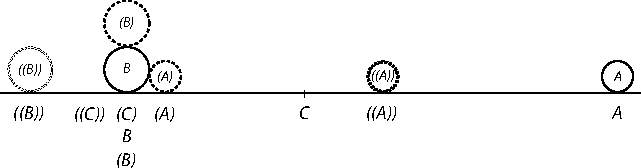
\includegraphics[width=0.98\textwidth]{gesamttex/edit_VIII,3/images/LH_35_09_23_004-005_d2.pdf}}%
  \vspace{0.5em}
  \centerline{\lbrack\textit{Fig.~2}\rbrack}%
%  \label{LH_35_09_23_004v_Fig.2}%
%  \vspace{2.0em}%
  \newpage%
%
%
\pstart%
\noindent%
\textit{A(A)} aequ. \textit{e}
aequ. \textit{AB}
aequ. \textit{A(B)}
aequ. \textit{A(C)}.
\rule[-3mm]{0pt}{0mm}%
%
\quad
$\displaystyle\frac{AC}{BC \sqcap c}$
aequ. $\displaystyle\frac{b}{a}.$
%
$AC + \underset{\displaystyle c}{CB}$ aequ. \textit{e}.
%
\textit{AC} aequ.
\rule[-3mm]{0pt}{9mm}%
$\displaystyle\frac{b}{a}\textit{BC}$
aequ. $\displaystyle\frac{b}{a}c.$
%
\textit{AC} aequ. $e - BC$
aequ. $e - c.$
%
\quad
Ergo \rule[-3mm]{0pt}{9mm}%
$\displaystyle\frac{b}{a}BC$
aequ.
$\displaystyle\underset{\displaystyle e-c}{e-BC}$
seu \textit{e} aequ.
$\overline{\displaystyle\frac{b}{a}+1}\,\underset{\displaystyle c}{BC},$
seu $\underset{\displaystyle c}{BC}$
aequ.
% \rule[1mm]{0pt}{5,0mm}%
$\displaystyle\frac{e}{1 + \displaystyle\frac{b}{a}}.$
%
Seu \textit{BC} aequ.
\rule[1mm]{0pt}{5,0mm}%
$\displaystyle\frac{a}{a+b}e$
aequ. \textit{c}
aequ.
%
\edtext{\textit{C(C)},
et \textit{AC}}{%
\lemma{\textit{C(C)}}\Bfootnote{\hspace{-0,5mm}%
\textbar~aequ. \textit{c} \textit{erg. u. gestr.}~%
\textbar~, et \textit{AC}%
~\textit{L}}}
%
aequ. $\displaystyle\frac{b}{a+b}e.$
\rule[-6mm]{0pt}{-6mm}%
\pend%
%
\pstart%
\textit{(B)((B))} aequ. \textit{y}.
\quad
\textit{(A)((A))} aequ.
%
\edtext{\lbrack$\epsilon$\rbrack.}{%
\lemma{\textit{e}}\Bfootnote{%
\textit{L~ändert Hrsg. nach~E,\cite{01056} S.~90}}}
%
\quad
$y + \epsilon$ aequ. $\delta.$%
\rule[-2mm]{0pt}{0mm}
% \pend%
% %
% \pstart%
\quad
$\kappa$ aequ.
%
\edtext{\textit{(C)((C))}. 
\quad
\textit{((B))((C))}}{%
\lemma{\textit{(C)((C))}.}\Bfootnote{\hspace{-0,5mm}%
\textbar~Constat autem esse $yb + a\epsilon$ aequ. \textit{ae}. \textit{gestr.}~%
\textbar\ \textit{((B))((C))}%
~\textit{L}}}
%
aequ. $\displaystyle\frac{a}{a+b}\delta.$
\rule[-1mm]{0pt}{7mm}%
\quad
\textit{((A))((C))} aequ. $\displaystyle\frac{b}{a+b}\delta.$
\quad
%
$\textit{(B)((B))} - \textit{((B))((C))}$ aequ.
\edtext{\textit{(B)((C))} seu aequ. \textit{(C)((C))}.}{%
\lemma{\textit{(B)((C))} \lbrack...\rbrack\ \textit{(C)((C))}}\Cfootnote{%
Die Gleichsetzung dieser Abstände entspricht der Annahme,
dass der Schwerpunkt sich nach dem Stoß gleichmäßig in dieselbe Richtung fortbewegt wie zuvor.
Im Folgenden wird diese Annahme widerlegt.}}
%
\quad
Ergo \rule[-1mm]{0pt}{7mm}%
$y-\displaystyle\frac{a}{a+b}\delta$ aequ $\kappa,$
seu $y-\displaystyle\frac{a}{a+b}\,\overline{y+\epsilon}$ aequ $\kappa,$
seu \rule[-2mm]{0pt}{8mm}%
$\displaystyle\frac{\raisebox{-3.0mm}{{\def\firstcircle{(0,0) circle (0.35cm)}\begin{tikzpicture}\draw \firstcircle node {\textit{ay}};\end{tikzpicture}}}+by\raisebox{-3.0mm}{{\def\firstcircle{(0,0) circle (0.35cm)}\begin{tikzpicture}\draw \firstcircle node {$-ay$};\end{tikzpicture}}}-a\epsilon}{a+b}$ aequ $\kappa,$
%
seu $\kappa$ aequ. \rule[-3mm]{0pt}{8mm}%
$\displaystyle\frac{by-a\epsilon}{a+b}.$
%
\quad
At supra \textit{c} aequ. $\displaystyle\frac{ae}{a+b}.$
%
Ergo
%
\edtext{si $\kappa$ aequ.~\textit{c},}{%
\lemma{si $\kappa$ aequ.~\textit{c}}\Cfootnote{%
Siehe die Erläuterung zu S.~\refpassage{LH_35_09_23_005r_dfgal-1}{LH_35_09_23_005r_dfgal-2}.}}
%
erit $by - a\epsilon$ aequ \textit{ae}.%
\rule[-2mm]{0pt}{7mm}%
\quad
Atqui si eaedem vires\protect\index{Sachverzeichnis}{vis servata} servantur,
erit $by + a\epsilon$ aequ. \textit{ae}.
Unde foret $-\,a\epsilon$ aequ. $+\,a\epsilon,$
quod est absurdum.%
\protect\index{Sachverzeichnis}{absurdum}
\rule[-1mm]{0pt}{6mm}%
\pend%
%
\pstart%
%
\edtext{Adeoque%
\edlabel{LH_35_09_23_004v_motusperpetuus_nnxh-1}
positis his duobus,
corpus minus incurrens%
\protect\index{Sachverzeichnis}{corpus incurrens}%
\protect\index{Sachverzeichnis}{corpus minus in majus}%
}{%
\lemma{Adeoque}\Bfootnote{%
\textit{(1)}~si incu
\textit{(2)}~positis his % duobus, corpus 
\lbrack...\rbrack\ minus incurrens%
~\textit{L}}}
%
\rule[-2mm]{0pt}{7mm}%
in majus quiescens%
\protect\index{Sachverzeichnis}{corpus quiescens}%
\protect\index{Sachverzeichnis}{corpus majus quiescens}
repelli,
%
\edtext{et centrum}{%
\lemma{et}\Bfootnote{\textbar~posito \textit{streicht Hrsg.}~\textbar\ centrum%
~\textit{L}}}
%
gravitatis eandem servare directionem,%
\protect\index{Sachverzeichnis}{directio centri gravitatis}
sequitur motus perpetuus artificialis,%
\protect\index{Sachverzeichnis}{motus perpetuus artificialis}
quod sic ostendo:
%
$by - a\epsilon$ non potest esse aequale ipsi $by + a\epsilon,$
sed est aequale ipsi $by + a\epsilon - 2 a\epsilon.$
%
Ergo si $by - a\epsilon$ aequ. \textit{ae},
erit et $by + a\epsilon - 2 a\epsilon$ aequ. \textit{ae}.
$by + a\epsilon$ aequ. $ae + 2 a\epsilon.$
%
Est autem $+\, ae$ vis ante concursum,%
\protect\index{Sachverzeichnis}{vis ante concursum}
et $by + a\epsilon$ vis post concursum,
ergo vis post concursum%
\protect\index{Sachverzeichnis}{vis post concursum}
major est quam \textit{ae}
(\protect\vphantom)%
quippe aequalis ipsi $ae + 2 a\epsilon$%
\protect\vphantom()
major inquam est vi ante concursum
%
\edtext{et excessus est $2 a\epsilon,$
seu vis}{%
\lemma{et}\Bfootnote{%
\textit{(1)}~vis
\textit{(2)}~excessus est $2 a\epsilon,$ seu vis%
~\textit{L}}}
%
repulsae duplicata.%
\protect\index{Sachverzeichnis}{vis repulsae}
Quod si ergo
%
\edtext{corpora servant eandem}{%
\lemma{corpora}\Bfootnote{%
\textit{(1)}~idem
\textit{(2)}~servant eandem%
~\textit{L}}}
%
viam%
\protect\index{Sachverzeichnis}{via centri gravitatis}
%
\edtext{et celeritatem%
\protect\index{Sachverzeichnis}{celeritas centri gravitatis}%
}{%
\lemma{et}\Bfootnote{%
\hspace{-0,5mm}celeritatem
\textit{erg.~L}}}
%
centri gravitatis%
\protect\index{Sachverzeichnis}{centrum gravitatis}
ante et post concursum,
et si corpus minus incurrens in majus quiescens,
repellitur,%
\protect\index{Sachverzeichnis}{corpus minus repulsum}
sequitur motus perpetuus artificialis,%
\protect\index{Sachverzeichnis}{motus perpetuus artificialis}
seu augmentum Virium,%
\protect\index{Sachverzeichnis}{augmentum virium}
quod est absurdum.%
\protect\index{Sachverzeichnis}{absurdum}
\pend%
%
\pstart%
Videamus an
%
\edtext{distantia%
\protect\index{Sachverzeichnis}{distantia corporum}}{%
\lemma{distantia}\Cfootnote{%
Gemeint ist der Abstand zwischen beiden Körpern nach dem Stoß.}}
%
esse possit eadem:
$y + \epsilon$ aequ. $\delta,$ et \textit{d} aequ \textit{e},
ergo $y + \epsilon$
%
\edtext{aequ. \textit{e}, ergo $ay + a\epsilon$ aequ \textit{ae},}{%
\lemma{aequ. \textit{e},}\Bfootnote{%
\textit{(1)}~rursus $yb + a\epsilon$ aequ. \textit{ae}
\textit{(2)}~ergo $ay + a\epsilon$ aequ \textit{ae},%
~\textit{L}}}
%
at si eaedem manent vires
erit $by + a\epsilon$ aequ. \textit{ae},
quare $ay + a\epsilon$ aequ. $by + a\epsilon,$
seu \textit{ay} aequ.\! \textit{by},
seu \textit{a} aequ.\! \textit{b}.
Quod est contra hypothesin,%
\protect\index{Sachverzeichnis}{hypothesis}
ponitur enim \textit{b} majus quam \textit{a}.
\pend%
%
\pstart%
Hinc patet\lbrack:\rbrack\
%
\edtext{si distantia%
%
\protect\index{Sachverzeichnis}{distantia corporum}
eadem maneat}{%
\lemma{si}\Bfootnote{%
\textit{(1)}~augeretur
\textit{(2)}~distantia eadem maneat%
~\textit{L}}}
%
corpore minore in majus incurrente,%
\protect\index{Sachverzeichnis}{corpus minus in majus}
et repulso,%
\protect\index{Sachverzeichnis}{corpus minus repulsus}
etiam haberi motum perpetuum,%
\protect\index{Sachverzeichnis}{motus perpetuus artificialis}
%
\edtext{nam $by + a\epsilon$ vis}{%
\lemma{nam}\Bfootnote{%
\textit{(1)}~posito
\textit{(2)}~$by + a\epsilon$
\textit{(a)}~virtus
\textit{(b)}~vis%
~\textit{L}}}
%
quaesita post concursum%
\protect\index{Sachverzeichnis}{vis post concursum}
major utique quam $ay + a\epsilon,$
id est
(\protect\vphantom)%
ex posita $y + \epsilon$ aequ. \textit{e},
seu ex hypothesi servatae%
\protect\index{Sachverzeichnis}{hypothesis}%
\protect\index{Sachverzeichnis}{distantia servata}
%
\edtext{distantiae%
\protect\vphantom()
quam}{%
\lemma{distantiae\protect\vphantom()}\Bfootnote{%
\textit{(1)}~major qua
\textit{(2)}~quam%
~\textit{L}}}
%
\textit{ae},
id est major
%
\edtext{quam vis}{%
\lemma{quam}\Bfootnote{%
\textit{(1)}~virtus
\textit{(2)}~vis%
~\textit{L}}}
%
quae erat ante concursum.%
\protect\index{Sachverzeichnis}{vis ante concursum}
Quod est absurdum.%
\protect\index{Sachverzeichnis}{absurdum}%
\edlabel{LH_35_09_23_004v_motusperpetuus_nnxh-2}%
\edlabel{LH_35_09_23_004-005_Blatt4v-2}
%
% \edtext{}{%
% \lemma{\textit{Am Rand:}}\Afootnote{%
% Demonstratio: quod in casu incursus corporis minoris\protect\index{Sachverzeichnis}{corpus minor} in majus et ab eo nonnihil repulsi impossibile est distantiam, \textsuperscript{[a]} corporum inter se eandem manere certo intervallo ante et post concursum; item quod iisdem positis impossibile est eandem manere viam centri gravitatis. Posito eandem manere quantitatem motus.%
% % \newline%
% % \newline%
% % {\footnotesize \textsuperscript{[a]} est
% % \textit{(1)}~vel distantiam, vel etiam
% % \textit{(2)}~distantiam,%
% % ~\textit{L}}
% }} 
%
\lbrack5~v\textsuperscript{o}\rbrack% % % %  Blatt 5v
%
\pend%
\vspace{1.5em}
% \newpage%
%
%
\pstart%
\noindent%
\lbrack\textit{Nachträglich (\glqq post reformationem\grqq) hinzugefügt:}\rbrack\
\pend%
\vspace{0.5em}
%
\pstart%
\noindent%
Videamus%
\edlabel{LH_35_09_23_004-005_Blatt5v-1}
vero quid prodeat,
quando non eadem quantitas motus,%
\protect\index{Sachverzeichnis}{quantitas motus}
attamen eo quo
%
\edtext{alibi}{%
{\lemma{alibi}\Bfootnote{%
\textit{erg.~L}}}%
{\lemma{alibi}\Cfootnote{%
Wohl in N.~\ref{dcc_08}, %??S01\textsubscript{10}, 
S.~\refpassage{LH_37_05_086r_reformatio_idzg-1}{LH_37_05_086r_reformatio_idzg-2}.
Siehe zur Textgenese von N.~\ref{dcc_02-2} die editorische Vorbemerkung, S.~\refpassage{dcc_intro_II-II_gdr-1}{dcc_intro_II-II_gdr-2}.%
}}}
%
explicui modo,
eadem vis servari debet,%
\protect\index{Sachverzeichnis}{vis servata}
tunc enim quadrata celeritatum%
\protect\index{Sachverzeichnis}{quadratum celeritatis}
duci debent in corpora.%
%
\edtext{}{%
\lemma{\textit{Am Rand, gestr.:}}\Afootnote{%
{\footnotesize%
Ergo $2ba \ \groesser \, b^2 - a^2$ ergo \textit{b} major \textit{a}.}}}
%
Et fiet aequatio:%
\protect\index{Sachverzeichnis}{aequatio}
$by^2 + a\epsilon^2$ aequ. $ae^2.$
%
At cum centrum gravitatis idem manet,%
\protect\index{Sachverzeichnis}{centrum gravitatis}
fit
$by-a\epsilon$ aequ. \textit{ae},
fiet
\textit{by} aequ. $a\,\overline{e +\epsilon}$
et
$by^2$ aequ. $a\,\overline{e^2-\epsilon^2}.$
%
Ergo \rule[-2mm]{0pt}{8mm}$\displaystyle\frac{by^2}{by}$ aequ. \rule[-2mm]{0pt}{8mm}$\displaystyle\frac{e^2-\epsilon^2}{e+\epsilon}.$ %
Ergo \textit{y} aequ. $e - \epsilon,$
sive $\epsilon + y$ aequ. \textit{e},
quae est corporum distantia.%
\protect\index{Sachverzeichnis}{distantia corporum}
\pend%
%
\pstart%
Ergo vim corporum eandem servari,%
\protect\index{Sachverzeichnis}{vis corporis}%
\protect\index{Sachverzeichnis}{vis servata}
et distantiam ante et post concursum,%
\protect\index{Sachverzeichnis}{distantia ante et post concursum}
idem est,
%
\edtext{quod servari simul.}{%
\lemma{quod}\Bfootnote{%
\textit{(1)}~vim se
\textit{(2)}~servari simul.%
~\textit{L}}}
%
\pend%
%
\pstart%
Itaque si haec duo conjungantur%
\lbrack,\rbrack\
via eadem centri gravitatis,%
\protect\index{Sachverzeichnis}{via centri gravitatis}
%
\edtext{et servatio ejusdem}{%
\lemma{et}\Bfootnote{%
\textit{(1)}~eadem
\textit{(2)}~servatio ejusdem%
~\textit{L}}}
%
distantiae%
\protect\index{Sachverzeichnis}{distantia corporum}%
\protect\index{Sachverzeichnis}{distantia servata}%
\lbrack,\rbrack\
hinc etiam colligitur eandem vim manere%
\lbrack:\rbrack\
sit enim
$y + \epsilon$ aequ. \textit{e}
et
$by - a\epsilon$ aequ. \textit{ae},
patet
\textit{y} aequ. $e - \epsilon$
et
\textit{by} aequ. $a\epsilon + ae,$
fiet
$by^2$ aequ. $ae^2 - a\epsilon^2$
sive
$ae^2$ aequ $by^2 + a\epsilon^2.$
\pend%
\newpage
\pstart%
Hinc patet vim
%
\edtext{percussionis effectum%
\protect\index{Sachverzeichnis}{effectus}%
\protect\index{Sachverzeichnis}{vis percussionis}
suum ostendere}{%
\lemma{percussionis}\Bfootnote{%
\textit{(1)}~esse
\textit{(2)}~effectum suum ostendere%
~\textit{L}}}
%
in separatione corporum.%
\protect\index{Sachverzeichnis}{separatio corporum}
Esse autem vim%
\protect\index{Sachverzeichnis}{vis percussionis}
%
\edtext{percussionis in iisdem
in ratione appropinquationum,%
\protect\index{Sachverzeichnis}{ratio appropinquationis}%
}{%
\lemma{percussionis in}\Bfootnote{%
\textit{(1)}~ratione
\textit{(2)}~iisdem
\textit{(a)}~corporis
\textit{(b)}~in ratione appropinquationum%
~\textit{L}}}
%
nec referre
%
\edtext{\lbrack utrum\rbrack}{%
\lemma{utrum}\Bfootnote{%
\textit{erg. Hrsg.}}}
%
majus sit corpus an minus,%
\protect\index{Sachverzeichnis}{corpus majus}%
\protect\index{Sachverzeichnis}{corpus minus}
quod movetur, quoad ictum,%
\protect\index{Sachverzeichnis}{ictus}
uti idem ictus est sive ego muro incurram,%
\protect\index{Sachverzeichnis}{murus}
sive murus mihi pari celeritate.%
\protect\index{Sachverzeichnis}{celeritas ictus}
Est autem vis percussionis tanta quanta esset,%
\protect\index{Sachverzeichnis}{vis percussionis}
si eadem corpora,
eadem
%
\edtext{celeritate appropinquationis%
\protect\index{Sachverzeichnis}{celeritas appropinquationis}%
}{%
\lemma{\textit{Am Rand, wohl auf} celeritate \textit{bezogen:}}\Afootnote{%
appropinquationis apparente%
\protect\index{Sachverzeichnis}{celeritas apparens}}}
%
aequali utique vi concurrerent.%
\protect\index{Sachverzeichnis}{vis concursus}
\pend%
%
\pstart%
Sint
%
\edtext{corpora \textit{a}, \textit{b},
quiescat}{%
\lemma{corpora}\Bfootnote{%
\hspace{-0,5mm}\textit{a}, \textit{b}, \textbar\ eorum momenta $e^2, i^2,$ celeritates \textit{e}. \textit{i} \textit{gestr.}~%
\textbar\ quiescat%
~\textit{L}}}
%
\textit{b} et \textit{a} feratur celeritate \textit{e}.
Ponamus concurrere vi%
\protect\index{Sachverzeichnis}{vis concursus}
%
\edtext{quae sit aequalis,}{%
\lemma{quae}\Bfootnote{%
\hspace{-0,5mm}sit
\textit{(1)}~\textbar~in \textit{streicht Hrsg.}~\textbar\ ratione
\textit{(2)}~aequalis%
~\textit{L}}}
%
nempe $am^2$ aequ. $bn^2,$
ita ut sit
$m + n$ aequ. \textit{e}.
Erit vis supposita
%
\edtext{$am^2 + bn^2.$
Est autem $e^2$ aequ. $m^2 + n^2 + 2mn$}{%
\lemma{$am^2 + bn^2$}\Bfootnote{%
\textit{(1)}~conferatur cum $ae^2,$
seu scribatur $am^2 + bn^2$
seu $am^2 + bn^2$ aequ. $ae^2\pleibdashv g^3.$
$am + an$ aequ. \textit{ae} seu $ae - am$ aequ. \textit{an} et $bn^2 \pleibvdash g^3$ aequ. $ae^2-am^2.$ Ergo $\displaystyle\frac{bn^2}{ae}$ aequ.
\textit{(2)}~. Est autem $e^2$ aequ. $m^2 + n^2 + 2mn$%
~\textit{L}}}
%
et
$ae^2$ aequ. $am^2 + an^2 + 2amn.$
Unde si auferatur
$am^2 + bn^2,$
restabit
$an^2 - bn^2 + 2amn$ aequ. $\pleibdashv g^3$
seu $\overline{a-b}\,n^2 + 2amn.$
%
Est autem \textit{m} aequ. $n\sqrt{\displaystyle\frac{b}{a}}.$
% \rule[-0mm]{0pt}{2mm}
Ergo fiet $\overline{\overline{a-b}\,+2a\sqrt{\displaystyle\frac{b}{a}}}\,n^2.$
\pend%
% \vspace{1.0em}
%
\pstart%
% \noindent%
% \lbrack\textit{Am Rand fortgesetzt:}\rbrack\ %
% \pend%
% % \vspace{0.5em}
%
% \pstart%
% \noindent%
$am^2$ aequ. $bn^2.$
%
Ergo \textit{m} aequ. $n\sqrt{\displaystyle\frac{b}{a}}$ et $m + n$ aequ. \textit{e}.
Ergo $\overline{1 + 1 \sqrt{\displaystyle\frac{b}{a}}}\,n$ aequ. \textit{e}.
Ergo $e^2$ aequ. $n^2 + 2n^2\sqrt{\displaystyle\frac{b}{a}}+\displaystyle\frac{b}{a}n^2$
et $ae^2$ aequ. $an^2 + bn^2+2n^2\sqrt{ab}.$
%
Comparetur cum $2bn^2,$
seu $a + b + 2\sqrt{ab}$
conferatur cum $2b,$
seu quad. ab $\sqrt{\protect\vphantom{b}a}+\sqrt{b},$
seu si
%
\edtext{$ae^2 \,\groesser\ am^2 + bn^2,$}{%
\lemma{$ae^2 \,\groesser$}\Bfootnote{\hspace{-0,5mm}%
\textit{(1)}~vi \textlangle per\textrangle\
\textit{(2)}~$am^2 + bn^2,$%
~\textit{L}}}
%
fiet etiam
$a+2\sqrt{ab}$ majus quam \textit{b},
seu $a + 2\sqrt{ab}$ aequ. $b + h.$
%
Ergo $a-b$ aequ.
%
\edtext{$h - [2] \sqrt{ab}$
vel}{%
\lemma{$h\,-$}\Bfootnote{\hspace{-0,5mm}%
\textbar~2 \textit{erg. Hrsg.}~%
\textbar\ $\sqrt{ab}$
\textit{(1)}~. Ergo
\textit{(2)}~vel%
~\textit{L}}}
%
$\pleibdashv a\ \pleibvdash b$ aequ. $\pleibdashv h\ \pleibvdash 2\sqrt{ab}.$
\quad
%
\edtext{Id est
si media proportionalis inter corpora duplicetur,}{%
\lemma{Id est}\Bfootnote{%
\textit{(1)}~rectangulum corporum duplicatum
\textit{(2)}~si media proportionalis inter corpora
\textit{(a)}~duplicata sit
\textit{(b)}~duplicetur,%
~\textit{L}}}
%
et ab ea unum corpus auferatur,
alterum vero ei addatur,
debet semper restare aliquid,
id est semper erit $a + 2\sqrt{ab}$
major quam \textit{b},
ergo
%
\edtext{\lbrack$6ab$\rbrack}{%
\lemma{$2ab$}\Bfootnote{%
\textit{L~ändert Hrsg.}}}
%
major quam $a^2 + b^2.$
%
\pend%
%
\pstart%
%
\edtext{Pro \textit{a} scribatur $\alpha^2,$
% \protect\rule[0mm]{0mm}{-4mm}%
pro \textit{b} scribatur $\beta^2,$}{%
\lemma{Pro \textit{a} \lbrack...\rbrack\ scribatur $\beta^2$}\Cfootnote{%
Die Setzungen $\displaystyle a = \alpha^2$ und $\displaystyle b = \beta^2$ werden im Folgenden nicht berücksichtigt.}}
%
fiet
%
\edtext{$a^2 + 2ba\ \groesser\, b^2.$
Ergo fiet et}{%
\lemma{$a^2 + 2ba\ \groesser\, b^2.$}\Bfootnote{%
\textit{(1)}~\textbar~sit \textit{streicht Hrsg.}~\textbar\ $a\ \groesser\, \displaystyle\frac{bg}{h}.$ Ergo fiet: $\displaystyle\frac{b^2g^2}{h^2}$
\textit{(2)}~. Ergo fiet et%
~\textit{L}}}
%
$a^2 + 2ab + b^2\ \groesser\, 2b^2,$
et $a + b\ \groesser\, b \sqrt{2},$
et $a\ \groesser\, \overline{\sqrt{2} - 1}\,b,$
seu
%
\edtext{$\displaystyle\frac{a}{b}\ \groesser\, \sqrt{2} - 1,$
quod non est universale,
imo falsum%
\protect\index{Sachverzeichnis}{falsum}
cum \textit{b} multo majus quam \textit{a}.}{%
\lemma{$\displaystyle\frac{a}{b}\ \groesser\, \sqrt{2} - 1,$}\Bfootnote{%
\textit{(1)}~quod est fa
\textit{(2)}~quod non % est universale, imo falsum 
\lbrack...\rbrack\ cum~\textit{b}
\textit{(a)}~$\groesser$~\textit{a}
\textit{(b)}~multo majus quam \textit{a}.%
~\textit{L}}}
%
Potest ergo fieri
ut vis percussionis%
\protect\index{Sachverzeichnis}{vis percussionis}
sit major tota vi,
quod videtur absurdum.%
\protect\index{Sachverzeichnis}{absurdum}%
\edlabel{LH_35_09_23_004-005_Blatt5v-2}
\pend%
\count\Bfootins=1200%
\count\Afootins=1200%
\count\Cfootins=1200%
%%
%\lbrack4~r\textsuperscript{o}\rbrack\  %%%% Blatt 4r
%%
%\pend%
%\vspace{1.0em}%
%%
%\pstart%
%\noindent%
%\lbrack\textit{Nachfolgend kleingedruckter Text in L gestrichen:}\rbrack\
%\pend%
%\vspace{0.5em}%
%%
%\footnotesize%
%\pstart%
%\noindent%
%$am^2$ aequ. $b^2.$
%\newline%
%\indent%
%Si ponamus viam centri gravitatis%
%\protect\index{Sachverzeichnis}{centrum gravitatis}
%manere eandem
%%\sout{et vero constat esse}
%pariter ac distantiam\lbrack,\rbrack\
%habebimus has duas aequationes
%%\sout{quando}
%$a\epsilon^2 + by^2$ aequ. $ae^2$ et \textit{a}
%\lbrack\textit{bricht ab.}\rbrack\ 
%\pend%
%\normalsize
%
%
%%%% Ende des Textes auf Bl. 5v.